  \documentclass{article}

\usepackage{textcomp}
\usepackage{enumitem}
\usepackage{soul}
\usepackage{tikz}
\usepackage{amsmath}
\usepackage{algorithm}
\usepackage{algpseudocode}
\setlistdepth{9}


%macros
\newcommand{\MovieL}{\textsc{MovieLens}}
\newcommand{\NetF}{\textsc{Netflix}}
\newcommand{\RecS}{\textsc{RecSys 2016}}
\newcommand{\Out}{\textsc{Outbrain}}
\newcommand{\ML}{\textsc{ML}}

\newcommand{\userS}{\mathcal{U}}
\newcommand{\itemS}{\mathcal{I}}
\newcommand{\vecU}{\mathbf{U}}
\newcommand{\vecI}{\mathbf{V}}
\newcommand{\MAP}{\texttt{MAP}}
\newcommand{\NDCG}{\texttt{NDCG}}

\newcommand{\RecNet}{\texttt{RecNet}}
\newcommand{\RecNetE}{{\RecNet}$_{E\!\!\backslash}$}
\newcommand{\MostPop}{\texttt{MostPop}}
\newcommand{\BPR}{\texttt{BPR-MF}}
\newcommand{\CoFactor}{\texttt{Co-Factor}}
\newcommand{\LightFM}{\texttt{LightFM}}


\newcommand{\Loss}{\mathcal{L}}
\newcommand{\Trn}{\mathcal{S}}


\newcommand{\D}{\mathcal D}
\newcommand{\EE}{\mathbb E}
\newcommand{\Ind}{\mathbbm{1}}

\newcommand{\N}{\mathbb N}
\newcommand{\Input}{\mathcal X}
\newcommand{\R}{\mathbb R}
\newcommand{\prefu}{\renewcommand\arraystretch{.2} \begin{array}{c}
   {\succ} \\  \mbox{{\tiny {\it u}}}
  \end{array}\renewcommand\arraystretch{1ex}}


\newcommand{\graph}{\Omega}
\newcommand{\graphH}{\mathcal H}

\newcommand{\vertices}{\mathcal V}
\newcommand{\edges}{\mathcal E}
\newcommand{\Cset}{\mathcal M}
\newcommand{\Weight}{W}
\newcommand{\cover}{\mathcal C}
\newcommand{\Xset}{\mathcal X}
\newcommand{\covers}{{\mathcal K}}
\newcommand{\bfZ}{\mathbf{z}}
\newcommand{\rademacher}{\mathfrak{R}}
\newcommand{\DA}{^\downarrow}

\newcommand{\kasandr}{\textsc{Kasandr}}

\newlist{myEnumerate}{enumerate}{9}
\setlist[myEnumerate,1]{label=(\arabic*)}
\setlist[myEnumerate,2]{label=(\Roman*)}
\setlist[myEnumerate,3]{label=(\Alph*)}
\setlist[myEnumerate,4]{label=(\roman*)}
\setlist[myEnumerate,5]{label=(\alph*)}
\setlist[myEnumerate,6]{label=(\arabic*)}
\setlist[myEnumerate,7]{label=(\Roman*)}
\setlist[myEnumerate,8]{label=(\Alph*)}
\setlist[myEnumerate,9]{label=(\roman*)}
\begin{document}
\begin{figure}[t!]
\begin{center}
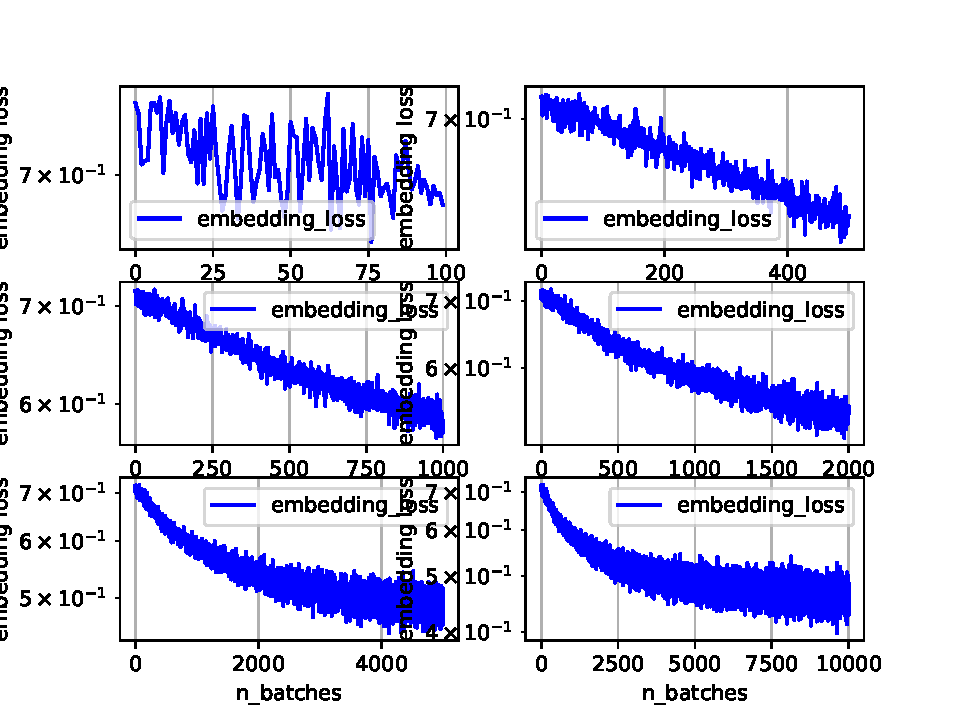
\includegraphics[width=1\textwidth]{figures/ml100k/embedding_loss_multipleplots.pdf}  
\end{center}
\caption{ml100k embedding loss with fixed alpha = 1.0}
\label{fig:ProperCover}
\end{figure}

\begin{figure}[t!]
\begin{center}
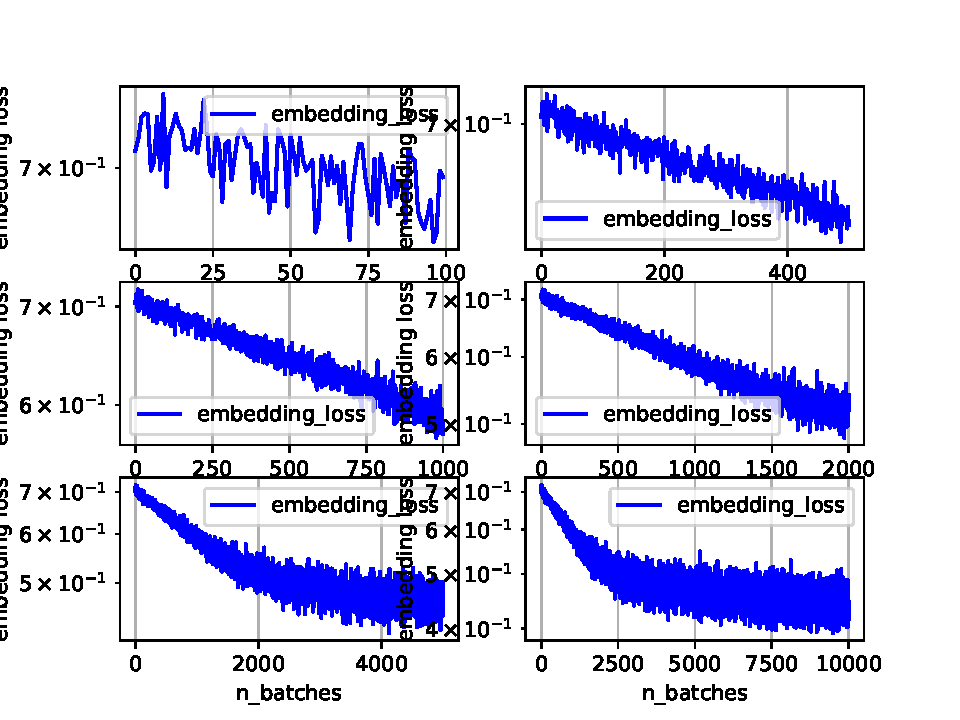
\includegraphics[width=1\textwidth]{figures/ml100k/embedding_loss_inc_alpha.pdf}  
\end{center}
\caption{ml100k embedding loss with increasing alpha. embedding loss does not seem to have converged}
\label{fig:ProperCover}
\end{figure}

\begin{figure}[t!]
\begin{center}
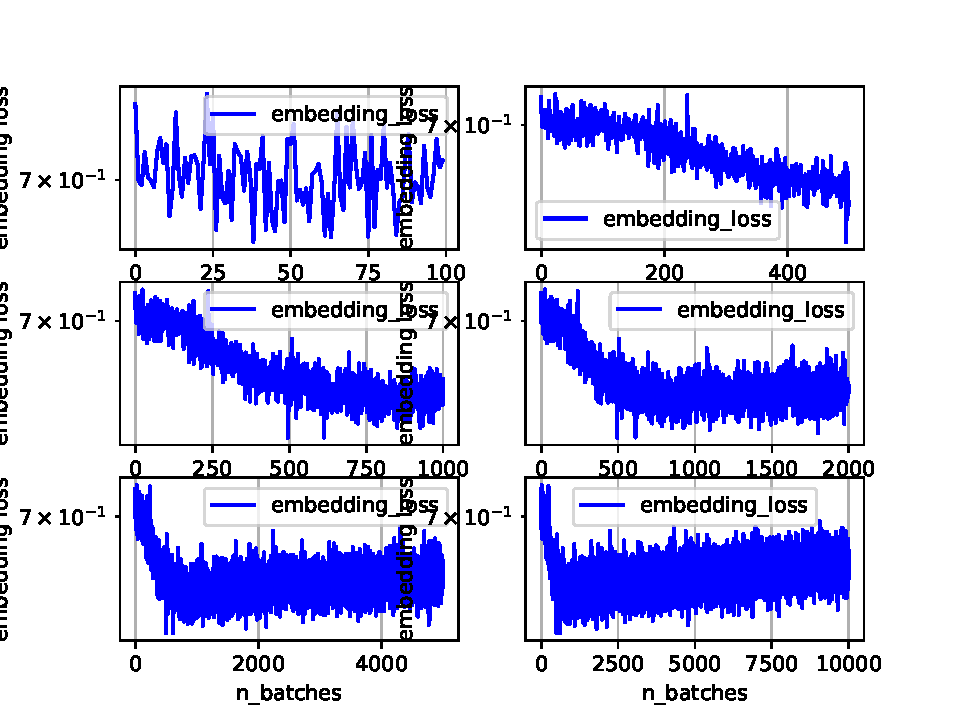
\includegraphics[width=1\textwidth]{figures/ml100k/embedding_loss_dec_alpha.pdf}  
\end{center}
\caption{ml100k embedding loss with decreasing alpha.}
\label{fig:ProperCover}
\end{figure}

\begin{figure}[t!]
\begin{center}
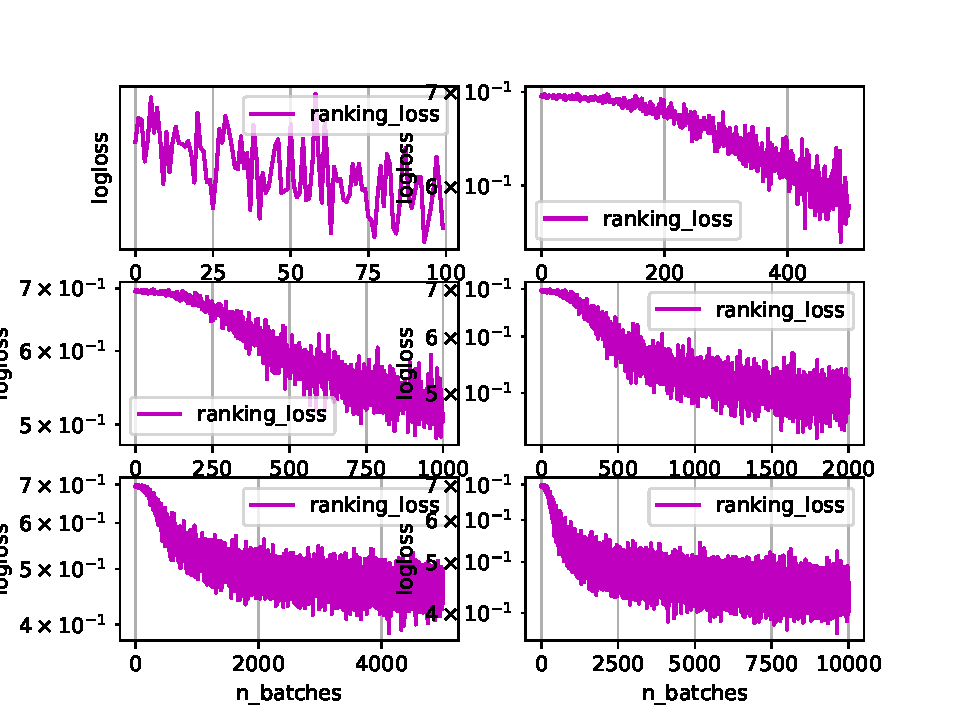
\includegraphics[width=1\textwidth]{figures/ml100k/ranking_loss_multipleplots.pdf}  
\end{center}
\caption{ml100k ranking loss with fixed alpha = 1.0}
\label{fig:ProperCover}
\end{figure}

\begin{figure}[t!]
\begin{center}
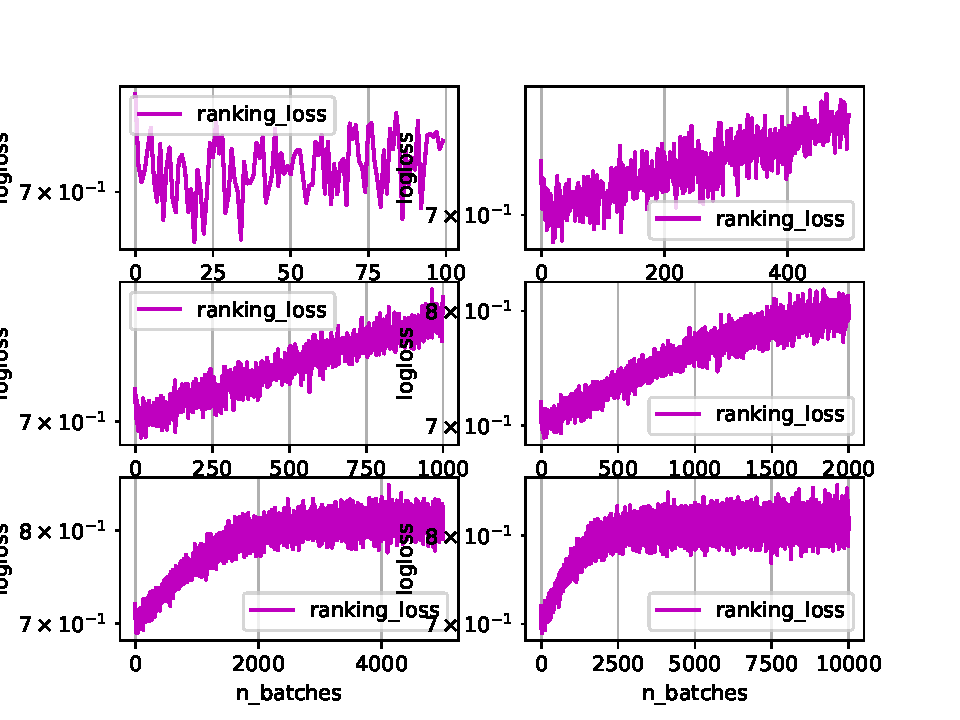
\includegraphics[width=1\textwidth]{figures/ml100k/ranking_loss_inc_alpha.pdf}  
\end{center}
\caption{ml100k ranking loss with increasing alpha. ranking loss does not seem to have converged}
\label{fig:ProperCover}
\end{figure}

\begin{figure}[t!]
\begin{center}
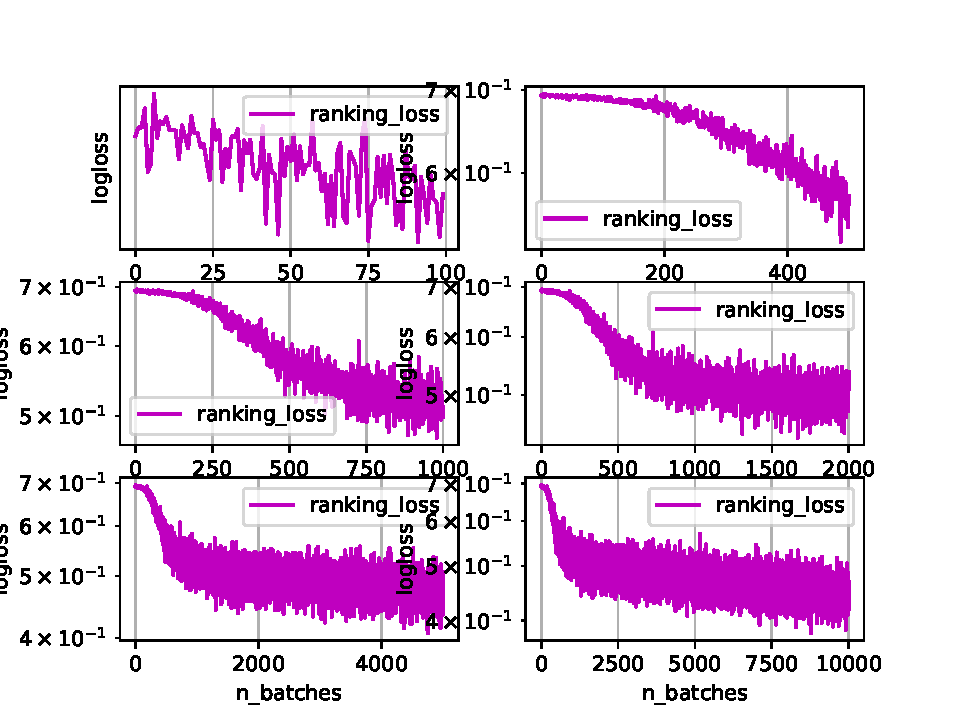
\includegraphics[width=1\textwidth]{figures/ml100k/ranking_loss_dec_alpha.pdf}  
\end{center}
\caption{ml100k ranking loss with decreasing alpha.}
\label{fig:ProperCover}
\end{figure}

\begin{figure}[t!]
\begin{center}
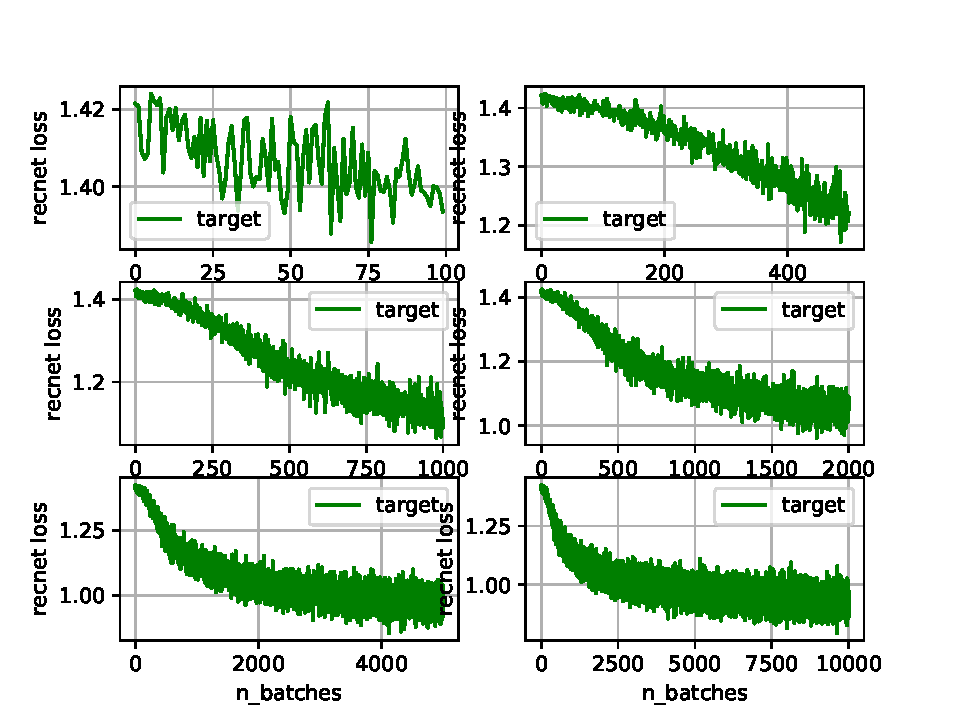
\includegraphics[width=1\textwidth]{figures/ml100k/target_loss_multipleplots.pdf}  
\end{center}
\caption{ml100k target loss with fixed alpha = 1.0}
\label{fig:ProperCover}
\end{figure}

\begin{figure}[t!]
\begin{center}
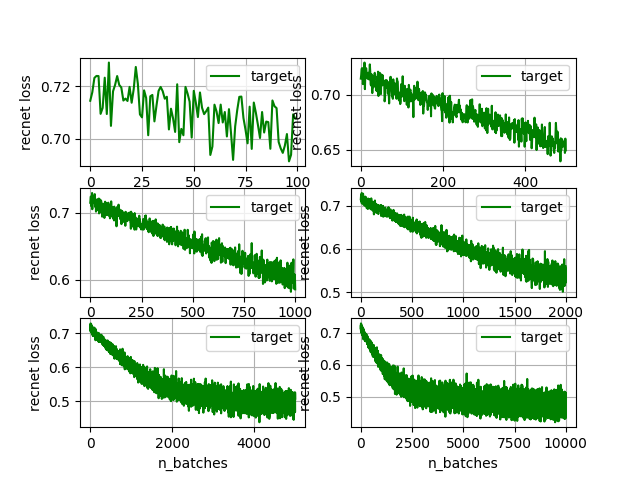
\includegraphics[width=1\textwidth]{figures/ml100k/target_loss_inc_alpha}  
\end{center}
\caption{ml100k target loss with increasing alpha. target loss does not seem to have converged}
\label{fig:ProperCover}
\end{figure}

\begin{figure}[t!]
\begin{center}
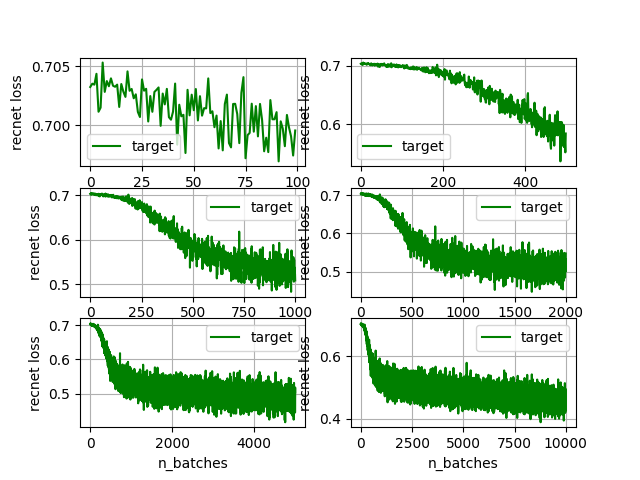
\includegraphics[width=1\textwidth]{figures/ml100k/target_loss_dec_alpha}  
\end{center}
\caption{ml100k target loss with decreasing alpha.}
\label{fig:ProperCover}
\end{figure}

\begin{table}[]
\centering
\caption{Results obtained on ML-100K. Settings with fixed $\alpha$, increasing $\alpha$ and decreasing $\alpha$}
\label{my-label}
\begin{tabular}{|c|c|c|c|}
\hline
                              & MAP@1 & MAP@5 & MAP@10 \\ \hline
$\alpha$ = 1.0, $\beta$ = 0.1 & 0.888 & 0.865 & 0.842  \\ \hline
Increase $\alpha$             &   0.819    &0.804       &   0.775     \\ \hline
Decrease $\alpha$             &   0.8375    &0.822       & 0.794       \\ \hline
\end{tabular}
\end{table}



\begin{table}[!b]
\centering
\caption{Results of all state-of-the-art approaches for implicit feedback when prediction is done only on offers shown to users. The best result is in bold, and a $\DA$ indicates a result that is statistically significantly worst than the best, according to a Wilcoxon rank sum test with $p < .01$.}
\label{tab:results_warm_interacted} 
\resizebox{\textwidth}{!}{\begin{tabular}{|c|cc|cc|cc|cc|}
\hline
                   & \multicolumn{2}{c|}{\ML-100K} & \multicolumn{2}{c|}{\ML-1M} & \multicolumn{2}{c|}{\NetF}& \multicolumn{2}{c|}{\kasandr}\\ \hline
            & MAP@1    & MAP@10 &MAP@1   & MAP@10&MAP@1   &MAP@10 & MAP@1   &  MAP@10 \\ \hline
%MostPop     & $0.633\DA$  &   $0.553\DA$  &$0.571\DA$&$0.553\DA$&$0.471\DA$&$0.480\DA$ &$0.037\DA$&$0.0383\DA$ \\ 
BPR-MF      & $0.613\DA$  &  $0.608\DA$   &$\textbf{ 0.788}$&$\textbf{0.748}$&$0.909\DA$&$0.842\DA$ &$0.857\DA$&$0.857\DA$     \\ 
LightFM        &     $0.772\DA$	    &    $0.770\DA$   &$0.832\DA$&$0.795\DA$&$0.800\DA$& $0.793\DA$ &$0.937\DA$&$0.936\DA$  \\ 
CoFactor          &      $0.718\DA$   &  $0.716\DA$        &$0.783\DA$&$0.741\DA$&$0.693\DA$&$0.705\DA$ &$0.925\DA$&$0.918\DA$\\ 
{\RecNet}$_c$      & $0.894\DA$    & $0.848\DA$  &$0.877\DA$&$0.835$&$0.877$&$0.846$&$0.958\DA$&$0.963\DA$  \\ 
{\RecNet}$_p$      &   $0.881\DA$  &   $0.846\DA$  &$0.876\DA$&$\textbf{0.839}$&$0.874$&$0.842$ &$0.915\DA$&$0.923\DA$      \\ 
{\RecNet}$_{c,p}$     &  $\textbf{0.888}$   & $\textbf{0.842}$       &$0.884\DA$&$\textbf{0.839}$&$\textbf{0.880}$&$\textbf{0.849}$ &$\mathbf{0.970}$&$\textbf{0.973}$   \\ \hline
\end{tabular}
}
\end{table}


\end{document}
